\documentclass[aspectratio=169,11pt]{beamer}

\usetheme{Madrid}
\usecolortheme{default}
\setbeamertemplate{navigation symbols}{}
\setbeamertemplate{footline}[frame number]
\setbeamertemplate{itemize items}[circle]

\usepackage{amsmath,amssymb,mathtools}
\usepackage{booktabs}
\usepackage{graphicx}
\usepackage{xcolor}
\usepackage{tikz}
\usepackage[T1]{fontenc}
\usepackage{lmodern}
\usepackage{appendixnumberbeamer}

\newcommand*{\bkmtranslateto}{\languagename}
\newcommand*{\bkmtranslate}[1]{%
  \ifcsname tr@@@\bkmtranslateto @#1\endcsname
    \csname tr@@@\bkmtranslateto @#1\endcsname
  \else
    #1%
  \fi
}
\pdfstringdefDisableCommands{%
  \let\translate\bkmtranslate
}

\newcommand{\iotaVec}{\mathbf{1}}
\newcommand{\Align}{\mathrm{Align}}

% Path to auto-generated regression tables (from scripts 63 and 64)
\newcommand{\tabledir}{../BNDES/output/muni_reg_tables}

\definecolor{darkblue}{RGB}{0,51,102}
\definecolor{alertred}{RGB}{180,30,30}
\definecolor{notegreen}{RGB}{0,100,50}

\setbeamercolor{frametitle}{fg=white}
\setbeamercolor{title}{fg=white}
\setbeamercolor{structure}{fg=darkblue}

\title{Progress Report --- First and Second-Stage Results}
% \subtitle{}
\author{}
\date{February 2026}

\begin{document}

% ===========================================================================
\begin{frame}
\titlepage
\end{frame}

% ===========================================================================
\begin{frame}{Research Question}

\textbf{Is the sector-level allocation of BNDES lending across municipalities GDP-optimal?}

\bigskip

\begin{itemize}
    \item BNDES disburses $\sim$3\% of GDP annually in subsidized industrial lending
    \item Existing literature (Lane 2025, Juh\'asz 2018) shows IP ``works'' for targeted sectors
    \item \textbf{But}: does the policymaker target the \emph{right} sectors?
    \item We derive and test the \textbf{first-order condition for optimality}: at an interior optimum, marginal reallocations across sectors have zero effect on GDP
\end{itemize}

\bigskip

\textbf{Contribution}: Move from ``does IP work?'' to ``is IP \emph{optimal}?''
--- and if not, identify which sectors are over/under-supported

\end{frame}

% ===========================================================================
\begin{frame}{Theory: Local Optimality Test}

Sector shares $s_m \in \Delta^{J-1}$, municipal output $Y_m = Y_m(s_m)$.

\medskip

\textbf{Directional derivative condition} --- at any interior optimum:
\begin{equation*}
    \frac{dY_m}{d\varepsilon}\bigg|_{\varepsilon=0}
    = \nabla_{s_m} Y_m \cdot v_m = 0
    \quad\text{for all } v_m \perp \iotaVec
\end{equation*}

\textbf{Empirical projection} (within-simplex, $\iotaVec'\Delta s_{mt}=0$):
\begin{equation*}
    \Delta Y_{m,t+h} = \beta' \Delta s_{mt} + u_{m,t+h}
\end{equation*}

\textbf{Null hypothesis (optimality)}:
\begin{equation*}
    H_0: \quad \beta = \mathbf{0}
\end{equation*}

\begin{itemize}
    \item Model-free: valid under any smooth objective
    \item $\hat\beta_j > 0$: sector $j$ under-supported $\implies$ tilt more toward $j$
    \item $\hat\beta_j < 0$: sector $j$ over-supported
\end{itemize}

\end{frame}

% ===========================================================================
\begin{frame}[allowframebreaks]{Identification: Shift-Share IV from Political Alignment}

$\Delta s_{mt}$ is endogenous $\implies$ need instruments that shift the sector mix exogenously.

\bigskip

\textbf{Shift} --- Political alignment turnover:
\begin{itemize}
    \item When party $p$ wins office $\ell \in \{\text{mayor, governor, president}\}$, BNDES credit tilts toward $p$-affiliated firms (Lazzarini et al.~2015, Carvalho 2014)
    \item $\Delta\Align^\ell_{mtp}$: party-$p$ alignment shock in municipality $m$, year $t$
\end{itemize}

\medskip

\textbf{Share} --- Baseline sectoral exposure to each party:
\begin{equation*}
    w_{mjp} \equiv \frac{\sum_{f \in (m,j)} L_{fp,t_0}}
    {\sum_{f \in (m,j)} N_{f,t_0}}
\end{equation*}
where $L_{fp}$ = number of owners of firm $f$ affiliated to party $p$; $N_f$ = total number of owners (affiliated and unaffiliated) of firm $f$.

\textbf{Instrument} (sector-specific, within municipality):
\begin{equation*}
    Z^\ell_{mjt} \equiv \sum_p w_{mjp} \cdot \Delta\Align^\ell_{mtp}
\end{equation*}

\medskip

{\footnotesize \textbf{Coverage}: 82.3\% of firm-muni-year rows have owner affiliation data ($N_f/F_f \approx 1.03$, near one owner per firm). At the sector-muni-year level, 74.5\% of cells have $\geq 1$ affiliated owner; the remaining 25.5\% receive $Z_{mjt} = 0$. These zero-instrument cells account for only 1.8\% of BNDES disbursement value.}

\end{frame}

% ===========================================================================
\begin{frame}{Estimation Strategy}

\textbf{First stage} (muni $\times$ sector $\times$ year):
\begin{equation*}
    \Delta s_{mjt} = \Pi Z_{mjt} + \alpha_{mj} + \alpha_{mt} + \eta_{mjt}
\end{equation*}
\begin{itemize}
    \item $\alpha_{mj}$: muni $\times$ sector FE \quad $\alpha_{mt}$: muni $\times$ year FE
    \item Muni$\times$year FE absorbs the \textbf{aggregate} political alignment shock
    \item Identification from \textbf{cross-sector variation} in party exposure $w_{mjp}$
\end{itemize}

\medskip

\textbf{Second stage} (muni $\times$ year, reduced form with sector-specific instruments):
\begin{equation*}
    \ln Y_{mt} = \sum_{j \neq j_0} \beta_j \widehat{\Delta s}_{mjt} +  \textcolor{red}{\psi \text{BNDES}_{mt}} + \delta_m + \delta_t + u_{mt}
\end{equation*}
\begin{itemize}
    \item $\beta_j$: GDP effect of reallocating 1pp from $j_0$ to sector $j$
    \item Control for $\text{BNDES}_{mt}$?: if instrument changes both composition and scale, controlling for scale may introduce bias.
    \item \textbf{Optimality test}: joint Wald $H_0: \beta = \mathbf{0}$
\end{itemize}

\end{frame}


% ===========================================================================
\begin{frame}{Data Sources}
\hypertarget{slide:datasources}{}

\begin{tabular}{lll}
\toprule
\textbf{Source} & \textbf{Content} & \textbf{Coverage} \\
\midrule
BNDES transparency portal & Loan-level disbursements & 2002--2024 \\
RAIS (MTE) & Employer-employee, CNAE sector & 2002--2017 \\
TSE / Colonnelli et al. & Worker affiliation \& donations (firm-level) & 2002--2019 \\
IBGE PIB Municipal & Municipality GDP & 2002--2017 \\
IBGE Population & Municipality population & 1991--2025 \\
IPCA (IBGE) & Price index for deflation & Base 2018 \\
SICONFI / basedosdados & Municipal transfers (placebo) & 2002--2017 \\
\bottomrule
\end{tabular}

\bigskip

\textbf{Geographic unit}: 5,570 valid municipalities \\
\textbf{Sector definition}: 21 CNAE 2.0 sections (letters A--U; \hyperlink{appendix:sectors}{\beamergotobutton{see distribution}})

\end{frame}

% ===========================================================================
\begin{frame}{Pipeline Architecture}

\begin{center}
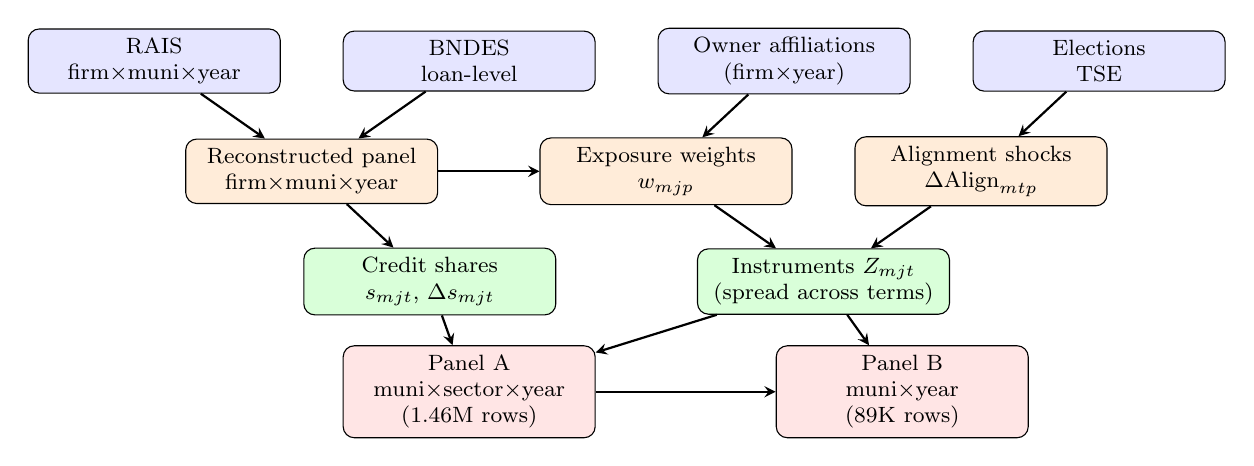
\begin{tikzpicture}[
    node distance=0.6cm and 1.2cm,
    box/.style={draw, rounded corners, minimum width=3.2cm, minimum height=0.7cm, font=\footnotesize, align=center},
    arrow/.style={->, thick, >=stealth}
]

% Row 1: Data inputs
\node[box, fill=blue!10] (rais) at (0,0) {RAIS\\firm$\times$muni$\times$year};
\node[box, fill=blue!10] (bndes) at (4,0) {BNDES\\loan-level};
\node[box, fill=blue!10] (owner) at (8,0) {Owner affiliations\\(firm$\times$year)};
\node[box, fill=blue!10] (elections) at (12,0) {Elections\\TSE};

% Row 2: Intermediate
\node[box, fill=orange!15] (recon) at (2,-1.4) {Reconstructed panel\\firm$\times$muni$\times$year};
\node[box, fill=orange!15] (weights) at (6.5,-1.4) {Exposure weights\\$w_{mjp}$};
\node[box, fill=orange!15] (shocks) at (10.5,-1.4) {Alignment shocks\\$\Delta\text{Align}_{mtp}$};

% Row 3: Instruments
\node[box, fill=green!15] (Z) at (8.5,-2.8) {Instruments $Z_{mjt}$\\(spread across terms)};
\node[box, fill=green!15] (shares) at (3.5,-2.8) {Credit shares\\$s_{mjt}$, $\Delta s_{mjt}$};

% Row 4: Panels
\node[box, fill=red!10] (panelA) at (4,-4.2) {Panel A\\muni$\times$sector$\times$year\\(1.46M rows)};
\node[box, fill=red!10] (panelB) at (9.5,-4.2) {Panel B\\muni$\times$year\\(89K rows)};

% Arrows
\draw[arrow] (rais) -- (recon);
\draw[arrow] (bndes) -- (recon);
\draw[arrow] (owner) -- (weights);
\draw[arrow] (recon) -- (weights);
\draw[arrow] (elections) -- (shocks);
\draw[arrow] (weights) -- (Z);
\draw[arrow] (shocks) -- (Z);
\draw[arrow] (recon) -- (shares);
\draw[arrow] (shares) -- (panelA);
\draw[arrow] (Z) -- (panelA);
\draw[arrow] (panelA) -- (panelB);
\draw[arrow] (Z) -- (panelB);

\end{tikzpicture}
\end{center}

\end{frame}

% ===========================================================================
\begin{frame}{Key Construction Decision: Instrument Timing}

\textbf{Problem}: Alignment shocks $\Delta\Align^\ell_{mtp}$ are only non-zero at inauguration years.
\begin{itemize}
    \item Mayors: 2005, 2009, 2013, 2017
    \item Governors/Presidents: 2003, 2007, 2011, 2015
    \item $\implies$ instruments zero for $\sim$70\% of panel
\end{itemize}

\bigskip

\textbf{Solution}: Spread each shock across the full 4-year electoral term.
\begin{itemize}
    \item Political alignment persists until the next election
    \item Mayor inauguration 2009 $\to$ shock applied to 2009, 2010, 2011, 2012
    \item Gov/Pres inauguration 2011 $\to$ shock applied to 2011, 2012, 2013, 2014
\end{itemize}

\bigskip

\textbf{After spreading}: Non-zero instruments for $\sim$65\% of muni-years (coalition instruments). Coverage: all years 2003--2017.

\end{frame}

% ===========================================================================
% FIRST-STAGE RESULTS (auto-generated from script 63)
% ===========================================================================

\begin{frame}{First Stage (Coalition): Single-Tier Instruments}

\begin{center}
\footnotesize
\begin{tabular}{lccc}
\toprule
& (1) Mayor & (2) Governor & (3) President \\
\midrule
$Z^{\text{mayor}}_{\text{coalition}}$ & $0.0282^{***}$ & & \\
& $(0.0080)$ & & \\[3pt]
$Z^{\text{gov}}_{\text{coalition}}$ & & $-0.0039$ & \\
& & $(0.0095)$ & \\[3pt]
$Z^{\text{pres}}_{\text{coalition}}$ & & & $-0.0225$ \\
& & & $(0.0151)$ \\
\midrule
Fixed Effects & $\alpha_{mj} + \alpha_{mt}$ & $\alpha_{mj} + \alpha_{mt}$ & $\alpha_{mj} + \alpha_{mt}$ \\
Clustering & muni + CNAE & muni + CNAE & muni + CNAE \\
Observations & 1,372,575 & 1,372,575 & 1,372,575 \\
$F$-statistic & \textbf{12.4} & 0.17 & 2.23 \\
\bottomrule
\end{tabular}
\end{center}

\begin{itemize}
    \item \textbf{Mayor alignment drives sector reallocation}: $F = 12.4$, passes Stock-Yogo threshold
    \item Interpretation: 1 s.d.\ mayor alignment shock $\to$ 2.8pp shift in sector share
\end{itemize}

\end{frame}

% ===========================================================================
\begin{frame}{First Stage (Party): Single-Tier Instruments}
\hypertarget{slide:fs-party-single}{}

\begin{center}
\footnotesize
\begin{tabular}{lccc}
\toprule
& (1) Mayor & (2) Governor & (3) President \\
\midrule
$Z^{\text{mayor}}_{\text{party}}$ & $0.0476^{***}$ & & \\
& $(0.0166)$ & & \\[3pt]
$Z^{\text{gov}}_{\text{party}}$ & & $-0.0314^{***}$ & \\
& & $(0.0101)$ & \\[3pt]
$Z^{\text{pres}}_{\text{party}}$ & & & $0.0601^{*}$ \\
& & & $(0.0337)$ \\
\midrule
Fixed Effects & $\alpha_{mj} + \alpha_{mt}$ & $\alpha_{mj} + \alpha_{mt}$ & $\alpha_{mj} + \alpha_{mt}$ \\
Clustering & muni + CNAE & muni + CNAE & muni + CNAE \\
Observations & 1,372,575 & 1,372,575 & 1,372,575 \\
$F$-statistic & \textbf{8.24} & \textbf{9.65} & 3.19 \\
\bottomrule
\end{tabular}
\end{center}

\begin{itemize}
    \item \textbf{Both mayor and governor individually significant} (unlike coalition)
    \item Party alignment is a more precise measure: fewer affiliated firms per party $\to$ sharper cross-sector variation
\end{itemize}
\vfill
\hfill\hyperlink{appendix:2002fixed}{\beamergotobutton{2002-fixed baseline}}
\end{frame}

% ===========================================================================
\begin{frame}{First Stage (Coalition): Combined Instruments}

\begin{center}
\footnotesize
\begin{tabular}{lccc}
\toprule
& (1) M+G & (2) M+P & (3) M+G+P \\
\midrule
$Z^{\text{mayor}}_{\text{coalition}}$ & $0.0287^{***}$ & $0.0251^{***}$ & $0.0252^{***}$ \\
& $(0.0069)$ & $(0.0065)$ & $(0.0054)$ \\[3pt]
$Z^{\text{gov}}_{\text{coalition}}$ & $0.0024$ & & $0.0006$ \\
& $(0.0084)$ & & $(0.0097)$ \\[3pt]
$Z^{\text{pres}}_{\text{coalition}}$ & & $-0.0184$ & $-0.0184$ \\
& & $(0.0141)$ & $(0.0147)$ \\
\midrule
Fixed Effects & $\alpha_{mj} + \alpha_{mt}$ & $\alpha_{mj} + \alpha_{mt}$ & $\alpha_{mj} + \alpha_{mt}$ \\
Clustering & muni + CNAE & muni + CNAE & muni + CNAE \\
Observations & 1,372,575 & 1,372,575 & 1,372,575 \\
Joint $F$ & \textbf{14.1} & 8.2 & \textbf{9.4} \\
$p$-value & $< 0.001$ & $< 0.001$ & $< 0.001$ \\
\bottomrule
\end{tabular}
\end{center}

\smallskip
\begin{itemize}\setlength{\itemsep}{0pt}
    \item Mayor instrument stable across specifications ($0.025$--$0.029$)
\end{itemize}

\end{frame}

% ===========================================================================
\begin{frame}{First Stage (Party): Combined Instruments}

\begin{center}
\footnotesize
\begin{tabular}{lccc}
\toprule
& (1) M+G & (2) M+P & (3) M+G+P \\
\midrule
$Z^{\text{mayor}}_{\text{party}}$ & $0.0454^{**}$ & $0.0480^{**}$ & $0.0459^{**}$ \\
& $(0.0164)$ & $(0.0169)$ & $(0.0168)$ \\[3pt]
$Z^{\text{gov}}_{\text{party}}$ & $-0.0266^{**}$ & & $-0.0239^{**}$ \\
& $(0.0098)$ & & $(0.0097)$ \\[3pt]
$Z^{\text{pres}}_{\text{party}}$ & & $0.0611^{*}$ & $0.0578$ \\
& & $(0.0348)$ & $(0.0359)$ \\
\midrule
Fixed Effects & $\alpha_{mj} + \alpha_{mt}$ & $\alpha_{mj} + \alpha_{mt}$ & $\alpha_{mj} + \alpha_{mt}$ \\
Clustering & muni + CNAE & muni + CNAE & muni + CNAE \\
Observations & 1,372,575 & 1,372,575 & 1,372,575 \\
Joint $F$ & \textbf{6.40} & 5.71 & \textbf{5.34} \\
$p$-value & $0.002$ & $0.003$ & $0.001$ \\
\bottomrule
\end{tabular}
\end{center}

\smallskip
\begin{itemize}\setlength{\itemsep}{0pt}
    \item Governor negative sign: winning party's sector loses share (crowd-out from other sectors?)
\end{itemize}

\end{frame}

% ===========================================================================
\begin{frame}[allowframebreaks]{Coalition vs.\ Party: Comparison}
\hypertarget{slide:comparison}{}

\begin{center}
\footnotesize
\begin{tabular}{lcccccc}
\toprule
& \multicolumn{3}{c}{\textbf{Coalition}} & \multicolumn{3}{c}{\textbf{Party}} \\
\cmidrule(lr){2-4} \cmidrule(lr){5-7}
& Coef & SE & $F$ & Coef & SE & $F$ \\
\midrule
\textbf{Single-tier (muni$\times$year FE):} & & & & & & \\[3pt]
Mayor & $0.028^{***}$ & $(0.008)$ & 12.4 & $0.048^{***}$ & $(0.017)$ & 8.2 \\
Governor & $-0.004$ & $(0.010)$ & 0.2 & $-0.031^{***}$ & $(0.010)$ & 9.7 \\
President & $-0.023$ & $(0.015)$ & 2.2 & $0.060^{*}$ & $(0.034)$ & 3.2 \\[6pt]
\textbf{Combined M+G+P:} & & & & & & \\[3pt]
Joint $F$ & \multicolumn{3}{c}{\textbf{9.4}} & \multicolumn{3}{c}{5.3} \\
$p$-value & \multicolumn{3}{c}{$< 0.001$} & \multicolumn{3}{c}{$0.001$} \\[6pt]
\textbf{Year FE robustness (M+G+P):} & & & & & & \\[3pt]
Joint $F$ & \multicolumn{3}{c}{\textbf{60.4}} & \multicolumn{3}{c}{28.5} \\
\bottomrule
\end{tabular}
\end{center}

\medskip

\begin{itemize}
    \item \textbf{Coalition}: stronger joint $F$ (9.4), concentrated in mayor tier
    \item \textbf{Party}: unlocks governor channel ($F = 9.7$), larger individual coefficients
    \item President sign flips: coalition negative vs.\ party positive
    \item \textcolor{alertred}{Take-away}: coalition preferred for joint $F$; party provides distinct variation at subnational tiers
\end{itemize}
\vfill
\hfill\hyperlink{appendix:ferobust}{\beamergotobutton{FE robustness}}

\end{frame}

% ===========================================================================
\begin{frame}{First-Stage Interpretation and Second-Stage Assumptions}

\textbf{What the first stage shows}:
\begin{itemize}
    \item Mayor alignment turnover shifts BNDES sector shares within municipalities
    \item Sectors with more party-affiliated firm owners gain relatively more credit
    \item Effect is $\sim$2.8pp per unit alignment shock, robust across specifications
\end{itemize}

\bigskip

\textbf{Key assumptions for second stage}:
\begin{enumerate}
    \item \textbf{Exclusion restriction}: Sector-specific $Z_{mjt}$ affects GDP \emph{only} through BNDES credit composition
    \begin{itemize}
        \item Concern: transfers, procurement, regulation also respond to alignment shocks
        \item Using sector-specific instruments helps: cross-sector variation in party exposure is less likely to correlate with transfers/procurement
        \item Planned test: show sector $Z$ does not predict municipal transfers
    \end{itemize}
    \item \textbf{Instrument relevance}: $F > 10$ (satisfied for mayor, borderline for all tiers)
    \item \textbf{SUTVA / no spillovers}: reallocation in muni $m$ doesn't affect muni $m'$
    \item \textbf{Local approximation}: perturbations are ``small'' (median $|\Delta s| \approx 0.02$)
\end{enumerate}

\end{frame}

% ===========================================================================
% SECOND-STAGE RESULTS (auto-generated from script 64)
% ===========================================================================

\begin{frame}{Second Stage: Reduced Form (Sector-Specific Instruments)}

\begin{center}
% Auto-generated Wald summary by script 64 (--specs=rf)
\begingroup
\centering
\begin{tabular}{lrrrrr}
\toprule
Specification & $N$ & $R^2$ & IVs & Wald $F$ & $p$-value \\
\midrule
Mayor & 89,008 & 0.9455 & 18 & 1.47 & 0.0894 \\
M+G & 89,008 & 0.9456 & 36 & 2.18 & $< 10^{-4}$ \\
M+G+bndes\_pc & 89,008 & 0.9456 & 36 & 2.18 & $< 10^{-4}$ \\
\bottomrule
\end{tabular}
\par\endgroup

\end{center}

\medskip

\begin{itemize}
    \item \textbf{Optimality null rejected}: M+G sector instruments jointly significant ($F = 2.18$, $p < 0.0001$)
    \item Mayor-only: marginal ($p = 0.09$); adding governor sector instruments sharpens rejection
    \item Adding $\text{bndes}_{pc}$ (scale control) makes no difference: $\approx 0$
\end{itemize}

\end{frame}

% ===========================================================================
\begin{frame}{Reduced Form: Notable Sector Coefficients}

From the M+G specification (36 sector-specific instruments, $F = 2.18$):

\bigskip

\begin{center}
\footnotesize
\begin{tabular}{llrl}
\toprule
\textbf{Sector} & \textbf{Tier} & \textbf{Coef (SE)} & \textbf{Sign.} \\
\midrule
C --- Manufacturing  & Mayor & $-0.080\;(0.038)$ & ** \\
P --- Education      & Mayor & $+0.390\;(0.096)$ & *** \\
M --- Professional   & Mayor & $+0.255\;(0.147)$ & * \\
S --- Other services & Mayor & $-0.478\;(0.280)$ & * \\
\midrule
E --- Water/waste    & Governor & $-0.462\;(0.135)$ & *** \\
I --- Accommodation  & Governor & $+0.372\;(0.145)$ & ** \\
P --- Education      & Governor & $+0.671\;(0.197)$ & *** \\
R --- Arts/recreation & Governor & $+0.213\;(0.079)$ & *** \\
\bottomrule
\end{tabular}
\end{center}

\medskip

\begin{itemize}
    \item Manufacturing (C) \textbf{over-supported}: reallocating toward C reduces GDP
    \item Education (P) \textbf{under-supported}: both mayor and governor channels show positive effect
    \item Coefficients relative to dropped sector G (wholesale/retail)
\end{itemize}

\end{frame}

% ===========================================================================
\begin{frame}{Second Stage: Robustness}

All robustness checks use M+G sector-specific instruments (36 IVs).

\bigskip

\begin{center}
% Auto-generated Wald summary by script 64 (--specs=robust)
\begingroup
\centering
\begin{tabular}{lrrrrr}
\toprule
Specification & $N$ & $R^2$ & IVs & Wald $F$ & $p$-value \\
\midrule
2002-fixed baseline & 89,008 & 0.9456 & 36 & 2.54 & $< 10^{-4}$ \\
Trimmed 1--99\% & 87,223 & 0.9466 & 36 & 2.04 & 0.0002 \\
Cluster: muni+year & 89,008 & 0.9456 & 36 & 1.71 & 0.0049 \\
\bottomrule
\end{tabular}
\par\endgroup

\end{center}

\bigskip

\begin{itemize}
    \item \textbf{Optimality rejection robust} across all specifications
    \item 2002-fixed baseline: strongest rejection ($F = 2.54$, $p < 0.0001$)
    \item Survives two-way clustering ($p = 0.005$) and trimming ($p = 0.0002$)
    \item Transfer placebo not yet available (SICONFI data insufficient)
\end{itemize}

\end{frame}

% ===========================================================================
\begin{frame}{Second Stage: Interpretation}

\textbf{Key insight}: Using sector-specific instruments isolates the BNDES composition channel.

\bigskip

\begin{itemize}
    \item \textbf{First stage}: Mayor alignment $\to$ BNDES sector reallocation ($\hat\Pi = 0.028^{***}$, $F = 12.4$)
    \item \textbf{Reduced form}: Sector-specific instruments jointly predict GDP ($F = 2.18$, $p < 0.0001$)
    \item $\implies$ \textbf{Optimality null rejected}: the current sectoral allocation is not GDP-optimal
\end{itemize}

\bigskip

\textbf{Policy-relevant sectors}:
\begin{itemize}
    \item Manufacturing (C): $\pi < 0$ --- over-funded relative to wholesale/retail
    \item Education services (P): $\pi > 0$ --- under-funded, strong signal from both tiers
    \item Water/waste (E, gov channel): $\pi < 0$ --- over-funded
\end{itemize}

\bigskip

\textbf{Next}: Vector 2SLS to estimate structural $\beta_j$ (sector-specific GDP elasticities) and test which sectors drive the rejection.

\end{frame}

% ===========================================================================
\begin{frame}{Additional Design Choices}

\footnotesize
\begin{center}
\begin{tabular}{@{}l p{10.5cm}@{}}
\toprule
\textbf{Choice} & \textbf{Description} \\
\midrule
Dropped sector & $j_0$ = G (Wholesale/retail trade), largest mean share (18.2\%). $\beta_j$ is relative to $j_0$. Joint test invariant to choice. \\[4pt]
Sparse sectors & T (Households as employers) and U (Extraterritorial) dropped: $<$100 nonzero instrument obs in 89K rows. Caused extreme leverage ($F = 82$ in 2002-fixed spec before dropping). \\[4pt]
Baseline weights & Primary: cycle-specific (last year before election). Robustness: 2002-fixed (all cycles use first year of data). \\[4pt]
Instrument def. & Currently: affiliated owner counts / total owners. Draft: employment-weighted within-sector party shares (TODO). \\
\bottomrule
\end{tabular}
\end{center}

\end{frame}

% ===========================================================================
\begin{frame}{Next Steps}

\textbf{Immediate}:
\begin{enumerate}
    \item Aggregate some sectors and re-run regressions
    \item Construct the employment-weighted instrument and re-run first and second stages
    \item Run scalar 2SLS (Table 5: $\Delta\text{HHI}$ instrumented by aggregate $Z$)
    \item Run vector 2SLS (Table 6: $\Delta s_j$ instrumented by sector $Z_j$) for structural $\beta_j$
    \item Transfer placebo (TODO: need to find data with better coverage)
\end{enumerate}


\end{frame}

% ===========================================================================
% APPENDIX
% ===========================================================================
\appendix

\begin{frame}{Appendix: Sector Share Distribution (with zeros)}
\hypertarget{appendix:sectors}{}

\footnotesize
\begin{center}
\begin{tabular}{lrrr}
\toprule
\textbf{CNAE Section} & \textbf{Mean $s_{mjt}$} & \textbf{\% Positive} & \textbf{$N$ obs} \\
\midrule
G --- Wholesale/retail trade & 0.182 & 38.9\% & 89,152 \\
C --- Manufacturing & 0.160 & 34.1\% & 85,008 \\
H --- Transport/storage & 0.123 & 30.8\% & 88,656 \\
A --- Agriculture & 0.036 & 11.1\% & 84,944 \\
F --- Construction & 0.024 & 12.9\% & 85,424 \\
J --- Information/communication & 0.024 & 8.3\% & 69,680 \\
B --- Mining & 0.023 & 9.9\% & 52,480 \\
N --- Admin services & 0.012 & 8.7\% & 84,944 \\
D --- Electricity/gas & 0.009 & 2.3\% & 35,696 \\
\emph{(12 sectors $<$ 1\%)} & \emph{$<$0.007} & \emph{$<$6\%} & --- \\
\bottomrule
\end{tabular}
\end{center}

\medskip

Total: 1,464,080 rows. 21 CNAE sections. 89.6\% of cells have zero BNDES credit.

Dropped sector $j_0$ = G (largest mean share).
\hfill\hyperlink{slide:datasources}{\beamerreturnbutton{Back to Data Sources}}

\end{frame}

% ===========================================================================
\begin{frame}{Appendix: First Stage --- 2002-Fixed Baseline Instruments}
\hypertarget{appendix:2002fixed}{}

\footnotesize
\begin{center}
\begin{tabular}{lcccccc}
\toprule
& \multicolumn{3}{c}{\textbf{Coalition}} & \multicolumn{3}{c}{\textbf{Party}} \\
\cmidrule(lr){2-4} \cmidrule(lr){5-7}
& Mayor & Governor & President & Mayor & Governor & President \\
\midrule
Coefficient & $0.0138^{**}$ & $-0.0093^{**}$ & $0.0051$ & $0.0102$ & $-0.0208^{***}$ & $0.0352$ \\
& $(0.0056)$ & $(0.0036)$ & $(0.0066)$ & $(0.0087)$ & $(0.0056)$ & $(0.0300)$ \\
$F$-stat & 5.98 & 6.49 & 0.59 & 1.40 & \textbf{13.9} & 1.38 \\
\midrule
\multicolumn{4}{l}{\textit{Coalition combined: $F = 6.73$, $p < 0.001$}}
& \multicolumn{3}{l}{\textit{Party combined: $F = 5.66$, $p < 0.001$}} \\
\bottomrule
\end{tabular}
\end{center}

\medskip

\begin{itemize}
    \item 2002-fixed baselines: clearly predetermined (first year of data)
    \item Coalition: mayor and governor individually significant
    \item Party: \textbf{governor is the strong instrument} ($F = 13.9$), mayor loses significance
    \item Pattern reversal from cycle-specific: party weights from 2002 are stale for mayor (shorter terms), but governor/president party structure more persistent
\end{itemize}
\vfill
\hfill\hyperlink{slide:fs-party-single}{\beamerreturnbutton{Back to First Stage}}

\end{frame}

% ===========================================================================
\begin{frame}[allowframebreaks]{Appendix: First Stage --- FE Robustness}
\hypertarget{appendix:ferobust}{}

\begin{center}
\footnotesize
\begin{tabular}{lcccc}
\toprule
& \multicolumn{2}{c}{\textbf{Coalition}} & \multicolumn{2}{c}{\textbf{Party}} \\
\cmidrule(lr){2-3} \cmidrule(lr){4-5}
& Muni$\times$yr FE & Year FE & Muni$\times$yr FE & Year FE \\
\midrule
$Z^{\text{mayor}}$ & $0.0252^{***}$ & $0.0228^{***}$ & $0.0459^{**}$ & $0.0430^{***}$ \\
& $(0.0054)$ & $(0.0019)$ & $(0.0168)$ & $(0.0148)$ \\[3pt]
$Z^{\text{gov}}$ & $0.0006$ & $0.0003$ & $-0.0239^{**}$ & $-0.0235^{**}$ \\
& $(0.0097)$ & $(0.0083)$ & $(0.0097)$ & $(0.0091)$ \\[3pt]
$Z^{\text{pres}}$ & $-0.0184$ & $-0.0160$ & $0.0578$ & $0.0519$ \\
& $(0.0147)$ & $(0.0120)$ & $(0.0359)$ & $(0.0353)$ \\
\midrule
Joint $F$ (M+G+P) & \textbf{9.4} & \textbf{60.4} & 5.3 & \textbf{28.5} \\
$p$-value & $< 0.001$ & $< 0.001$ & $0.001$ & $< 0.001$ \\
\bottomrule
\end{tabular}
\end{center}

\medskip

\begin{itemize}
    \item Coefficients robust across FE specifications within each alignment definition
    \item Year FE boosts $F$ substantially for both definitions (as expected)
    \item \textbf{Conservative choice}: muni$\times$year FE as primary; coalition for strongest joint $F$
    \item Party instruments useful as robustness check and for overidentification tests
\end{itemize}
\vfill
\hfill\hyperlink{slide:comparison}{\beamerreturnbutton{Back to Comparison}}

\end{frame}

\end{document}
